\documentclass{article}
\usepackage{graphicx}
\usepackage{pdfpages}
\usepackage{hyperref}
\usepackage{appendix}

\usepackage[printwatermark]{xwatermark}
\usepackage{xcolor}
\usepackage{graphicx}
\usepackage{lipsum}
\usepackage{amsmath}

\DeclareMathOperator*{\argmin}{argmin}

\begin{document}

\title{Accelerating layer-wise training and pruning for neural networks
with RELU link functions}
\author{David Johnston}

\maketitle

\begin{abstract}
Faster training of Neural Nets
\end{abstract}

\section{Problem statement}

We want to find the optimal weights for a neural network with one hidden layer
and a rectified linear unit RELU link function, $Max(0, x)$.

That is find

\[
\argmin_u ~ \lambda ~ ||u||_1 + \sum_p || Max(0, u^T x_p) - y_p||_2^2
\]

The variable $u$ is a matrix mapping the vector space of $x$ into the vector
space of $y$. The $p$ index indicates the different data points of the
training set. Each $(x_p, y_p)$ is a pair of vectors making up data-point $p$.
The L1 norm on $u$ is there to regularize and promote sparsity.

This minimization is separable over the $y$ dimension so, without loss of
generality, we can treat $y_p$ as scalars and $u$ as a vector.
When $y_p$ is negative these terms are convex. When $y_p$ is positive the
term is non-convex so in general, this is a non-convex optimization problem.
While it is non-convex and can have multiple local minima, the structure of
these RELU link functions make poor local minim rare. So finding the minimum
by gradient descent can work but it can be tricky due to the existence of
plateaus and ridges which can result in slow convergence.

Our goal is to try to solve this optimization problem taking advantage of the
simple structure and symmetries of the individual terms in order to arrive at an
algorithm which is more efficient and robust.

\section{Strategy}

We can solve non-convex problems using a few general strategies. One common
strategy is using a convex relaxation or (approximate thereof) and then
local methods to fine tune from there. The convex relaxation gives a lower
bound on the global optimum. Any current best solution gives an upper bound.
Note that our problem is unconstrained.

One method which is very powerful for solving non-convex problems is the
convex-concave procedure, CCP, which is also known by other names such as
difference of convex programming \cite{boyd-ccp}.

If a non-convex problem can be writtem as the difference of two convex
functions or, equivalently, the sum of a convex and a concave one, we can
define another function where we linearize the concave term around some point.
This function is now convex and is a \emph{majorization} of the original
functions. That is, it has the following two characteristics. 1) It is a convex
global upper bound on the function. 2) The value of the function and the first
derivative at the point majorized around, are equal to the non-convex function.
From this you can see that if you minimize the majorization, you have found a
local minimum of the non-convex function which is an upper bound on the global
minimum. Often, it will be the global minimum particularly when poor local
minima are rare.



Therefore, we can iteratively solve the majorized convex problem and then
re-majorize around the new solution. This procedure converges rapidly and when
it does, it means we have at least a local minima of the original non-convex
function.

\section{Convex relaxation and majorization}

The non-convex function is
\[
f(u) = \left (Max(0, u^T x) - y \right) ^2
\]

We will define $w = u^T x$ to simplify notation. So our full non-convex function is

\begin{eqnarray}
f(w) & = & \left (Max(0, w) - y \right) ^2 \\
 & = & y^2 + \theta(w) ~ (w^2 - 2~w~y)
\end{eqnarray}
where $\theta(z)$ is a Heaviside function, 1 if $z > 0$ and zero otherwise (it's value at z=0
won't matter for us).

This function is convex when $y<0$ so we only need to find a convex relaxation or
majorization when $y$ is positive.

The convex relaxation of this is
\[
f_r(w) = \theta(w-y)~(w - y)^2
\]

The majorization (via the CCP) around current point $w_0$ is a choice of two
functions depending on $w_0$.

\begin{eqnarray}
f_m(w) & = & (w - y)^2  ~ \mbox{~if~} w_0 \ge 0 \\
 & & (1-\theta(w-2y)) y^2 + \theta(w-2y)~(w - y)^2 ~ \mbox{~if~} w_0 < 0
\end{eqnarray}

See Figure 1 for an illustration of these functions.

\begin{figure}
  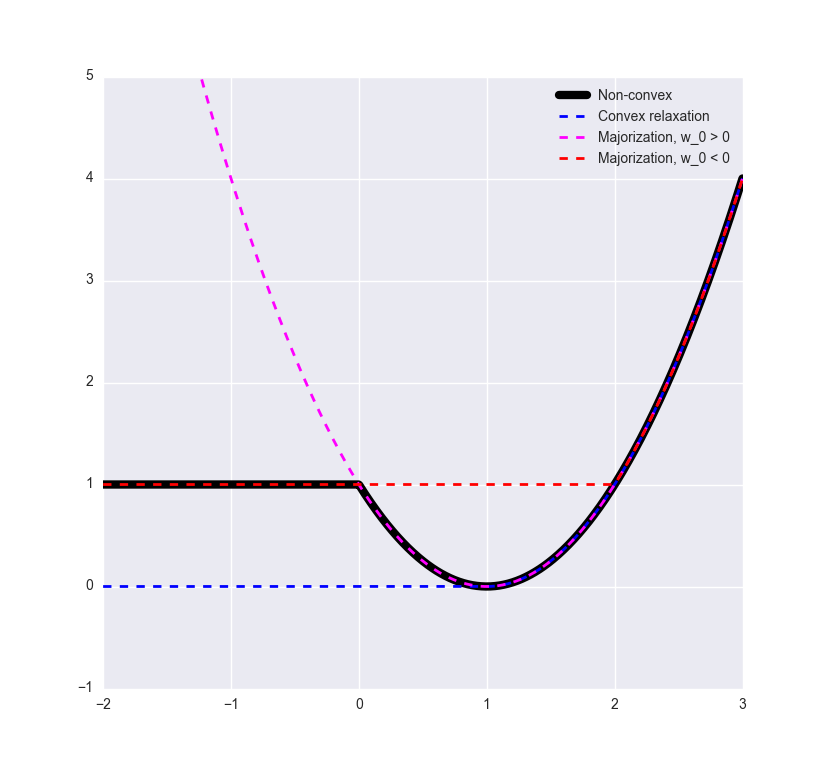
\includegraphics[width=\textwidth]{relax_maj.png}
  \caption{Shows the original non-convex function (when $y>0$),
  the convex relaxation and the
  majorization for either cases of CCP current value, $u_0$.}
\end{figure}


The majorization is always a convex function but is one of two functions
depending on the point we majorize around. As it converges, it will settle on
one of the functions. When it has settled on a function for all terms in the
sum over $p$, the entire process finishes. It typically converges in less than
10 iterations.

\section{Optimizing with ADMM}

So the convex optimizations for either relaxed or majorized problems reduces to
minimizing a sum of incomplete quadratic terms. They are
quadratic on only one side of the line and constant on the other side and
continuous at the boundary though not always differentiable at the boundary.
While they are quadratic functions, they only vary in one direction; the one
parallel to $x_p$. They are constant in the directions orthogonal to $x_p$.

If these terms were complete quadratics, the sum would itself be a quadratic
function and our problem would reduce to a L1 regularized least squares problem.
However, due to the incompleteness, minimizing the sum of these is more
complicated.

This sum of functions is still convex so any general purpose convex
optimization solver will work.

Our method of performing this optimizing efficiently uses the Alternative
Directions Method of Multipliers ADMM in consensus form \cite{boyd-admm}.
This is done as follows. We will optimize the sum as if each has it's own
independent $u_p$ and then constrain all of the $u_p$ to be equal. To do this
we add a Lagrange multiplier and another term which is the square of the
constraint. This is known as the augmented lagrangian method and the
iterative approach to solving it is ADMM.

The cost function we are trying to minimize in all cases can be written

\[
C(u) = \lambda ~ ||u||_1 + \sum_p \theta(u^T x_p - z_p) ~ Q(u^T x_p; y_p)
\]

where $Q$ is a general quadratic expression.

\[
Q(w; y) = w^2 - 2 w y
\]

For the purpose of optimization,
we can add or subtract a constant so we can restrict to quadratics that are zero
when the argument is zero.

We can make the $\theta$ function become unity by formally taking it's location parameter
$z$ to be $-\infty$.

Due to the $\theta$ functions. i.e. the incompleteness, we don't know of an analytic
expression for the argument which minimizes this function. However, we can derive an analytic
expression for it if there were only one data point. This motivates the application of ADMM
to the problem.

ADMM in the consensus form involves creating a unique variable $u_p$ corresponding to
each data point. This decouples all of the
sums. Then we constrain them to be equal through the use of a Lagrangian.
See \cite{boyd-admm}) chapter 7.

\[
L = \lambda ~ ||u||_1 + \sum_p \theta(u^T x_p - z_p) ~ Q(u_p^T x_p; y_p, c_p)
 ~ + ~ \frac{\rho}{2} ||u_p - u + d_p||_2^2
\]

where $d_p$ is a Lagrange multiplier or dual variable and $\rho$
is an algorithmic parameter akin to a step-size in gradient descent.
In consensus form, the iterations at step $k+1$ becomes

\begin{eqnarray}
u_p^{k+1} & = & \argmin_{~u_p} Q(u_p^T x_p; y_p) + \frac{\rho}{2} ||u_p - u^k + d_p^k||_2^2 \\
u^{k+1} & = & S_{\lambda / N \rho} (\bar{u}^{k+1} - \bar{d}^k) \\
d_p^{k+1} & = & d_p^k + u_p^{k+1} - u^{k+1} \\
\end{eqnarray}
The bars indicate average over the $p$. $N$ in the number of the $p$ indexed data points.
$S_\alpha(x)$ is the soft-thresholding function which is given by

\begin{eqnarray}
S_\alpha(x) & = & x - \alpha ~\mbox{if}~ x > \alpha \\
& = & 0 ~\mbox{if}~ |x| \le \alpha \\
& = & x + \alpha ~\mbox{if}~ x < -\alpha \\
\end{eqnarray}

\section{The proximal operator for incomplete quadratics}

The last remaining task is to perform the first minimization which is a sum of
a single incomplete quadratic function and a spherically symmetric complete quadratic.
Due to the symmetry, it's clear that this reduces down to a one-dimensional problem.
The minimum will occur either at the quadratic center or pushed in the direction of the
incomplete quadratic.

So we need to solve the problem

\[
x^* = \argmin_x \theta(x-z) (x^2 -2 x y) + \lambda (x-r)^2
\]

which is an evaluation of the proximal operator of the incomplete quadratic
function $\theta(x-z) (x^2 -2 x y)$. We can calculate this as follows. Clearly if
$r < z$ and the incomplete quadratic is flat at $r$, $x^*$ must be $r$.
Similarly if $r$ is much larger than $z$, the $\theta$ function is ignorable and
so we are just minimizing a quadratic whose minimum is a weighted average of the
two means, that is

\[
x^* = \frac{\lambda r + y}{1+\lambda}
\]

This will be the solution as long as $x^* > z$. Setting this expression to $z$
and solving for $r$ we get the other interesting value.

\[
r_U = \frac{(1+ \lambda)z -y}{\lambda}
\]

At both of these values, $x^*=z$, and because the proximal operator must be continuous and non-decreasing
$x^*$ must also be $z$ between these two points. So as a function of $v$, this proximal function looks
somewhat like the soft-thresholding function but with a slope change in the second sloping section.

So to summarize, the piecewise linear function for
$x^*$ is given by

\[
    x^*(r) = \begin{cases}
        r & \text{if } r < z \\
        z & \text{if } z \le r \le r_U\\
        (\lambda r + y)/(1+\lambda) & \text{if } r > r_U
        \end{cases}
  \]

\section{The full algorithm}

To summarize, we can separate and parallelize the minimization over the
dimension of $y$. For each of those we iterate over 10 or so CCP iterations,
$N_{CC}$. For each of those we iterate over 100 or so ADMM iterations, $N_A$.
Each ADMM iteration has complexity $N_x N$. So final complexity is
$N_x~N_y~N~N_{CC}~N_{A}$. Even with $N$ of a million, this can be computed in
less than a minute on a typical laptop when dimensions $N_x$ and $N_y$ are
not large. There are a few tricks to accelerate the algorithm and reduce the
number of ADMM iterations to a smaller number like 10.


\begin{figure}
  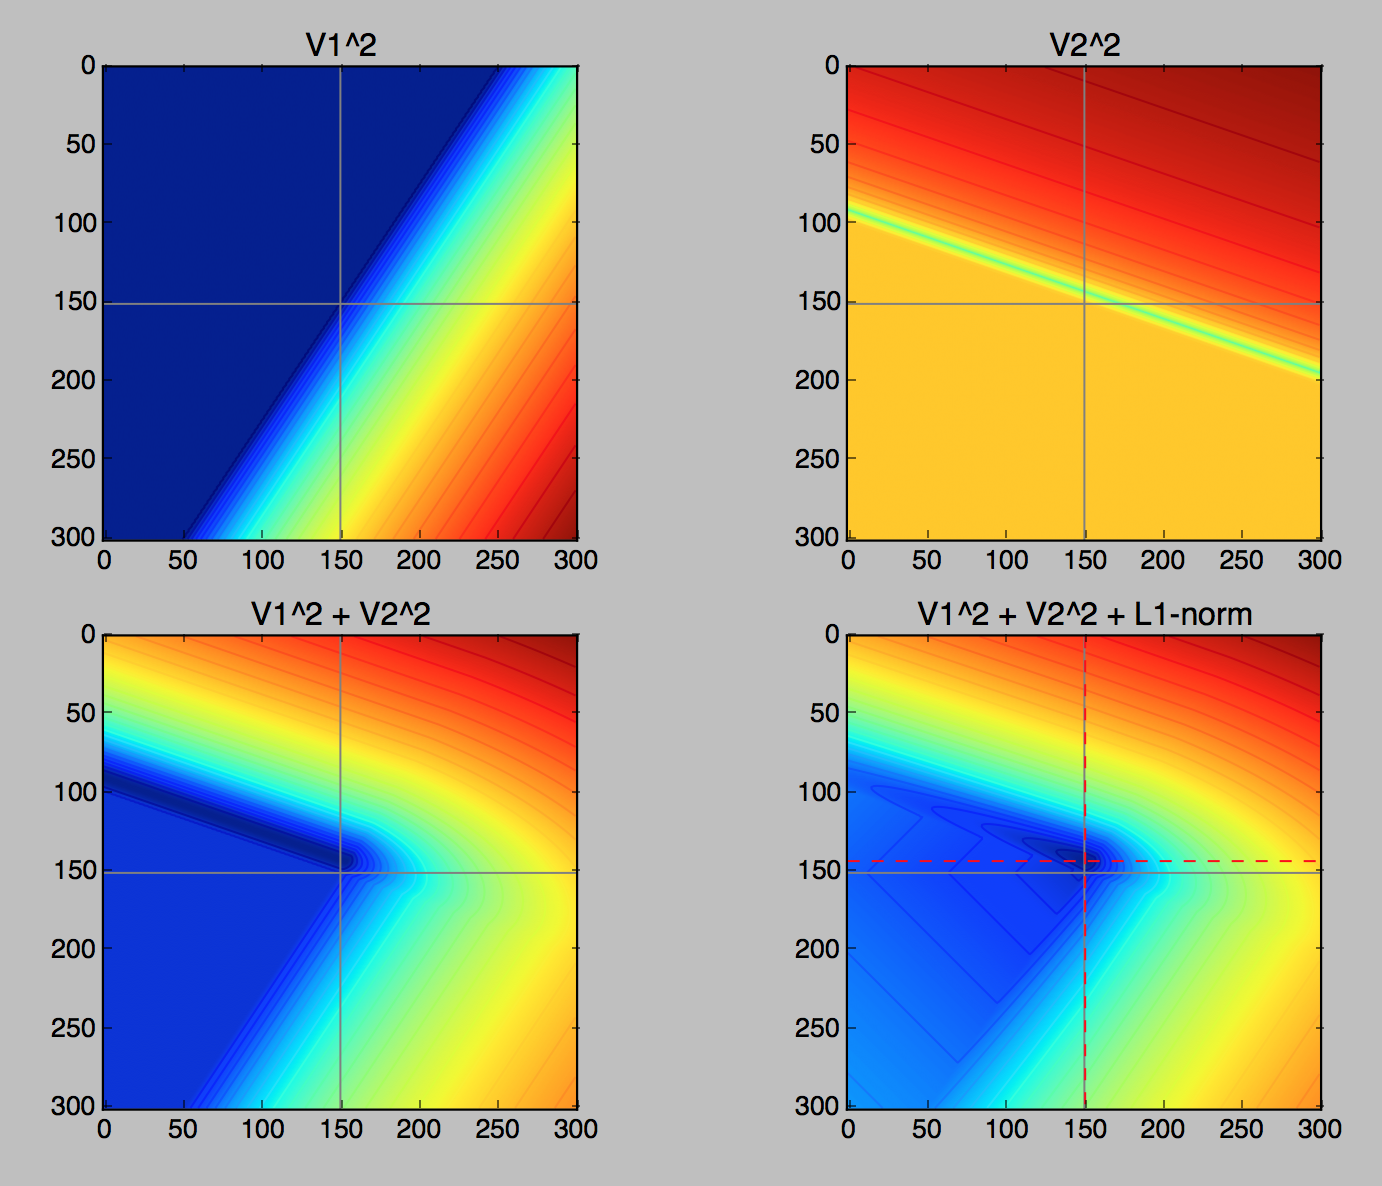
\includegraphics[width=\textwidth]{nc.png}
  \caption{Shows how two incomplete quadratics in 2D combine to form a more complicated function
  with broken symmetry and a unique local minimum. The goal of using ADMM is to decompose the minimization
  in order to exploit these symmetries.}
\end{figure}



\begin{thebibliography}{20}
\bibliographystyle{plain}

\bibitem{boyd-admm}
  Boyd S., Parakh N., Chu E., Peleato B. \& Eckstein J.,
  \emph{Distributed Optimization and Statistical Learning via the
  Alternating Direction Method of Multipliers},
Foundations and Trends in Machine Learning
Vol. 3, No. 1 (2010) 1–122 \\
{\url{http://stanford.edu/~boyd/papers/pdf/admm_distr_stats.pdf}}

\bibitem{boyd-proximal}
  Parakh N. \& Boyd S.,
  \emph{Distributed Optimization and Statistical Learning via the
  Alternating Direction Method of Multipliers},
Foundations and Trends in Optimization
Vol. 1, No. 3 (2013) 123–231 \\
{\url{https://web.stanford.edu/~boyd/papers/pdf/prox_algs.pdf}}

\bibitem{boyd-ccp}
  Parakh N. \& Boyd S.,
  \emph{Variations and Extension of the Convex-Concave Procedure},
Foundations and Trends in Optimization
Optimization and Engineering (online), November 2015.\\
{\url{http://stanford.edu/~boyd/papers/pdf/cvx_ccv.pdf}}

\bibitem{zheng-card}
  Zheng X., Sun  X., Li D. \& Sun J.
  \emph{Successive Convex Approximations to Cardinality-Constrained
  Quadratic Programs: A DC Approach},
  Tech. rep., School of Management, Fudan University; 2012.\\
{\url{http://www.optimization-online.org/DB_FILE/2012/04/3423.pdf}}

\bibitem{three-weight}
Derbinsky N., Bento J., Elser V., Yedidia J.
{\url{https://arxiv.org/abs/1305.1961}}


\bibitem{diamond}
  Diamond, S., Reza, T. \& Boyd, S.
  \emph{A General System for Heuristic Solution of Convex Problems over Nonconvex Sets},
{\url{http://www.optimization-online.org/DB_FILE/2012/04/3423.pdf}}

https://stanford.edu/~boyd/papers/pdf/ncvx.pdf

\end{thebibliography}

\end{document}
